\documentclass[11pt, a4paper]{article}

\usepackage[top=15mm, bottom=15mm, left=25mm, right=25mm]{geometry}
\usepackage{tikz}
\usepackage{amssymb,amsmath, amsthm}
\usepackage[labelsep=period]{caption}

\newtheorem{theorem}{Theorem}[section]
\newtheorem{corollary}{Corollary}[theorem]
\newtheorem{lemma}[theorem]{Lemma}

\newcommand{\Figure}[1]{Figure~\ref{#1}}
\newcommand{\Eq}[1]{Eq.~\ref{#1}}
\newcommand{\set}[1]{\mathbb{#1}}

\begin{document}
\title{Euler 94: Almost equilateral triangles}
\date{}
\author{Didier Pieroux}
\maketitle

\begin{abstract}
It is easily proved that no equilateral triangle exists with integral length sides and integral area. However, the almost equilateral triangle 5-5-6 has an area of 12 square units.

We shall define an almost equilateral triangle to be a triangle for which two sides are equal and the third differs by no more than one unit.

Find the sum of the perimeters of all almost equilateral triangles with integral side lengths and area and whose perimeters do not exceed one billion (1,000,000,000).
\end{abstract}

\section{Formulation}
Let consider an isosceles triangle of base $b\in\set N$, of equal sides $a\in\set N$, and of height $h$ (\Figure{fig:triangle1}).
  
\begin{figure}[h]
    \begin{center}
        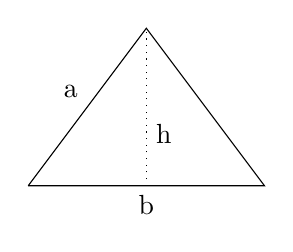
\begin{tikzpicture}[scale=0.5]
        \draw (0, 0) 
           -- (6, 0) node[midway, below] {b} 
           -- (3, 4) 
           -- (0, 0) node[midway, above left] {a} ;
        \draw[dotted] (3, 0) -- (3, 4) node[pos=0.33, right] {h};
        \end{tikzpicture}
        \caption{Geometric description}
        \label{fig:triangle1}
    \end{center}
\end{figure}

The problem is then described by the following equations, with $P$ the perimeter and $S$ the area:
\begin{align}
    a & = b \pm 1 \\ \label{eq:a1}
    P & = 2a+b \\ 
    S & = bh/2 \\
    a^2 & = (b/2)^2 + h^2 \label{eq:pytha1}
\end{align} 
    
\begin{lemma}$b$ is even.\end{lemma}
\begin{proof} Let suppose that $b$ is odd. For $S$ to be integral, $h$ must be an even integer: $h=2h'$ with $h'\in\set N$. But then $a^2 = b^2/4 + 4h'^2$ is not integral, `which contradicts the hypothesis that $a$ is integral.
\end{proof}

For ease, let us pose $b=2c$ with $c\in\set N$ (\Figure{fig:triangle2}). 
\begin{figure}
    \begin{center}
        \begin{tikzpicture}[scale=0.5]
        \draw              (0, 0) -- (3, 0) node[midway, below] {c};
        \draw [dashed] (3, 0) -- (6, 0) -- (3, 4);
        \draw              (3, 4) -- (0, 0) node[midway, above left] {a} ;
        \draw[dotted]      (3, 0) -- (3, 4) node[pos=0.33, right] {h};
        \end{tikzpicture}
        \caption{Reformulated geometric description}
        \label{fig:triangle2}
    \end{center}
\end{figure}

The equations (\ref{eq:a1})-(\ref{eq:pytha1}) read now:
\begin{eqnarray}
a & = & 2c \pm 1 \\
P & = & 2(a+c) \\ 
S & = & ch \\
a^2 & = & c^2 + h^2 
\end{eqnarray}

\section{Tree of primitive Pythagorean triples}
A Pythagorean triple $(a, b c)$ is a triple whose components are positive integers such that $a^2+b^2=c^2$. If the components have no common factor, the triple is said to be primitive. Obviously, given a primitive Pythagorean triple, an infinite number of Pythagorean triples can be generated by multiplying each components by a same positive integer. Reciprocally, any non-primitive Pythagorean triple can be reduced to a primitive one by dividing the components by their common factor.

Let us consider the following three matrices:
\[
A = \left(\begin{matrix}  1 & -2 & 2 \\  2 & -1 & 2 \\  2 & -2 & 3 \end{matrix} \right)\!,\ 
B = \left(\begin{matrix}  1 &  2 & 2 \\  2 &  1 & 2 \\  2 &  2 & 3 \end{matrix} \right)\!,\
C = \left(\begin{matrix} -1 &  2 & 2 \\ -2 &  1 & 2 \\ -2 &  2 & 3 \end{matrix} \right)\!.
\]

It can be shown that all primitive Pythagorean triples, and only them, are generated without duplication by recursively multiplying the first primitive Pythagorean triple, namely $p_0=(3, 4, 5)$, by each of these matrices\footnote{https://en.wikipedia.org/wiki/Tree\_of\_primitive\_Pythagorean\_triples}.

\end{document}
